\chapter{Pipeline d’extraction multimodale}
\label{chap:extraction}

\section{Introduction}\label{sec:c4-1}

Ce chapitre décrit comment on obtient, à partir d’un dossier scanné, la sortie brute du modèle multimodal, c’est-à-dire l’ensemble d’entités et de relations que la chaîne TRACE reçoit ensuite en entrée (chapitre~\ref{chap:architecture}). Il ne s’agit pas encore de réduire les hallucinations : l’objectif est de produire une extraction aussi complète que possible, mais construite selon des règles fixées à l’avance, pour que les erreurs mesurées ensuite soient bien celles du modèle.

Un principe guide toute cette étape : aucune règle de l’extraction ne s’appuie sur le Gold Standard. Les consignes données au modèle et les contrôles appliqués à ses réponses viennent uniquement du TRACE-Sepsis Annotation Guideline (chapitre~\ref{chap:donnees-gold}) et du texte de la page. Sans cette séparation, une partie des performances mesurées refléterait la connaissance de la référence plutôt que la qualité du modèle.

Le chapitre présente d’abord l’architecture générale du pipeline (section~\ref{sec:c4-2}) et la préparation des dossiers (section~\ref{sec:c4-3}). Il détaille ensuite la construction des prompts (section~\ref{sec:c4-4}), les modèles comparés (section~\ref{sec:c4-5}), l’extraction des entités et des relations (sections~\ref{sec:c4-6} et~\ref{sec:c4-7}) et le post-traitement des sorties (section~\ref{sec:c4-8}). Il expose enfin la manière dont les sorties sont comparées au Gold Standard (sections~\ref{sec:c4-9} et~\ref{sec:c4-10}) et le choix du modèle retenu pour TRACE (section~\ref{sec:c4-11}).

\section{Architecture générale du pipeline d’extraction}\label{sec:c4-2}

Le pipeline traite chaque dossier page par page. Pour chaque page, il enchaîne quatre opérations :

\begin{enumerate}
  \item la page du PDF est convertie en image ;
  \item le modèle lit l’image et en transcrit le texte ;
  \item à partir de ce texte, le modèle extrait les entités cliniques ;
  \item à partir du texte et de la liste des entités retenues, il extrait les relations.
\end{enumerate}

Chaque appel au modèle est suivi d’une validation déterministe : seules les entités retrouvées dans le texte de la page et les relations conformes au guideline sont conservées. Les résultats des pages sont ensuite réunis dans un fichier JSON par dossier, qui contient à la fois les annotations de chaque page et leur union à l’échelle du dossier. La figure~\ref{fig:c4-pipeline} résume cet enchaînement.

\begin{figure}[H]
\centering
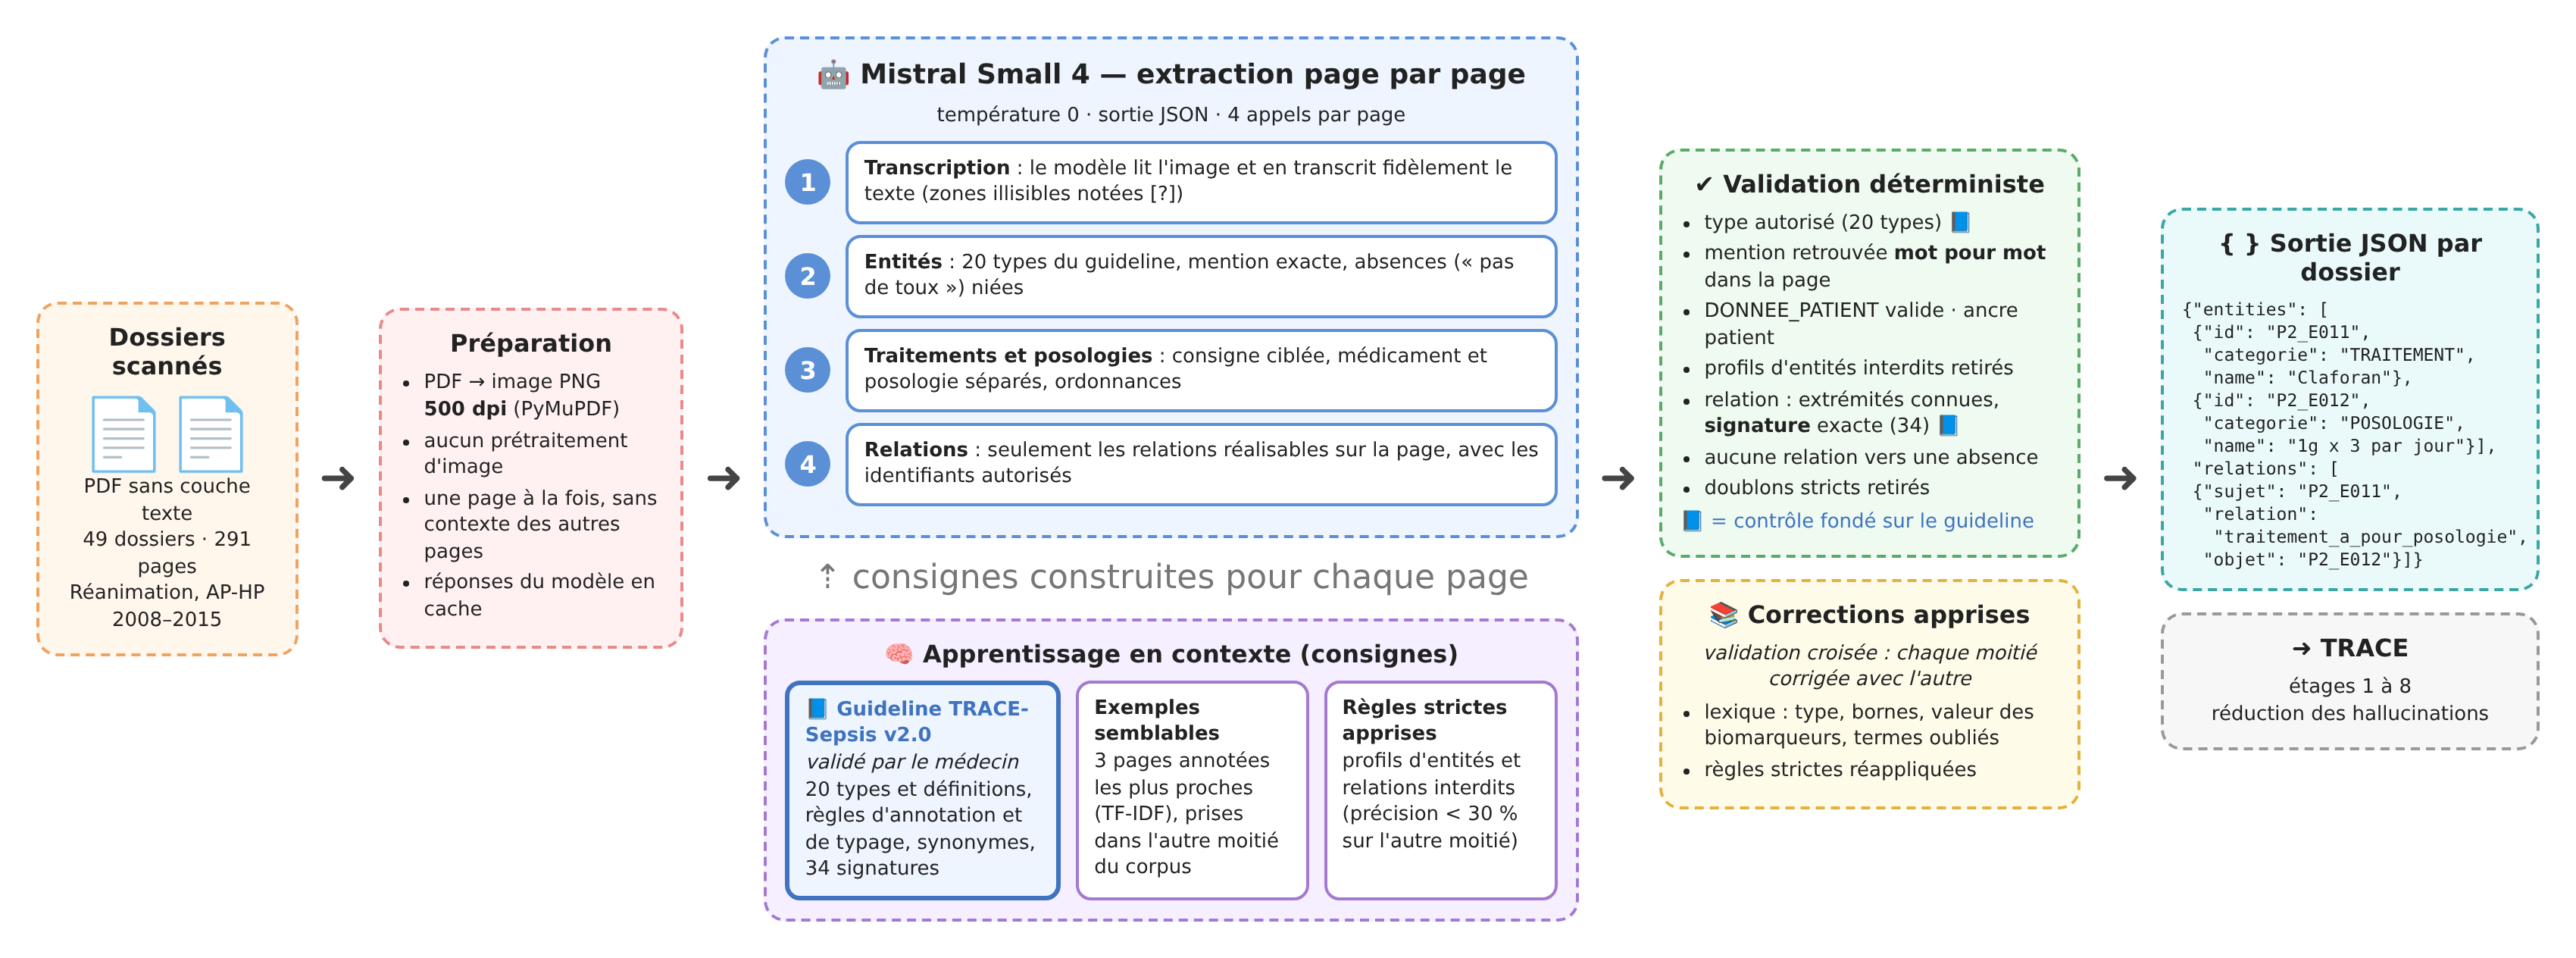
\includegraphics[width=\textwidth]{images/fig_pipeline_extraction.png}
\caption{Pipeline d’extraction multimodale, de la page scannée à la sortie JSON du dossier}\label{fig:c4-pipeline}
\end{figure}

Séparer la transcription, les entités et les relations en trois appels a deux avantages. Chaque consigne reste courte et ciblée, ce qui limite les oublis quand la page est dense. Surtout, les entités et les relations s’appuient sur un texte fixé une fois pour toutes, celui de la transcription : c’est ce texte qui sert ensuite à vérifier que chaque élément est bien écrit dans la page, ici comme dans la chaîne TRACE.

\section{Préparation des dossiers médicaux}\label{sec:c4-3}

\subsection{Conversion des PDF en images}\label{sec:c4-3-1}

Les dossiers sont des PDF issus de la numérisation de documents papier, sans couche texte (section~\ref{sec:c3-3-2-4}). Chaque page est convertie en image PNG avec la bibliothèque PyMuPDF, à une résolution de 500~points par pouce et sans canal de transparence. Cette résolution élevée a été choisie pour préserver les petits caractères, les tableaux de biologie et les valeurs numériques, qui sont précisément les informations les plus exposées aux erreurs de lecture. L’image est ensuite transmise au modèle encodée en base64.

\subsection{Prétraitement}\label{sec:c4-3-2}

Aucun prétraitement d’image n’est appliqué : pas de redressement, de débruitage ni de binarisation. Le texte n’est pas non plus extrait par un moteur d’OCR intermédiaire. Le modèle multimodal lit directement l’image de la page, ce qui évite d’accumuler les erreurs d’un OCR et celles du modèle de langage. Ce choix a une contrepartie : la qualité de la lecture dépend entièrement des capacités visuelles du modèle, et une page mal scannée n’est pas corrigée avant d’être lue.

\subsection{Gestion des documents multi-pages}\label{sec:c4-3-3}

Les dossiers comptent de 4 à 12 pages. Chaque page est traitée séparément, ce qui garde des consignes de taille raisonnable et permet de rattacher chaque information à la page d’où elle vient. Les entités reçoivent un identifiant qui contient le numéro de page (par exemple \texttt{P3\_E012}), et les relations un identifiant unique dans le dossier.

Le revers de ce découpage est qu’une relation dont les deux extrémités sont sur des pages différentes ne peut pas être extraite. Le cas existe, par exemple lorsqu’un germe est identifié sur une page et l’antibiotique adapté prescrit sur une autre. Cette limite est assumée : elle est le prix de la traçabilité, et elle est mesurée par le rappel des relations.

Toutes les réponses du modèle sont mises en cache, indexées par le contenu exact de la requête. Une interruption, fréquente sur une API publique, ne fait donc pas perdre le travail déjà fait, et une relance produit exactement les mêmes sorties.

\section{Prompt engineering}\label{sec:c4-4}

\subsection{Guideline-guided prompting}\label{sec:c4-4-1}

Les consignes ne sont pas écrites à la main pour l’extraction : elles sont générées automatiquement à partir du fichier du guideline. Pour chaque type d’entité, le prompt reprend sa description, ses valeurs autorisées et ses notes ; il reprend aussi les règles générales d’annotation, les règles de typage (signe vital ou symptôme, symptôme ou défaillance, traitement administré ou envisagé, diagnostic ou foyer infectieux…) et la table des synonymes. Pour les relations, il liste les 34 signatures avec leur domaine, leur portée et leur description.

Cette construction garantit que le modèle reçoit les mêmes définitions que l’annotatrice. Elle évite aussi d’introduire, au fil des essais, des consignes ajustées sur les erreurs observées dans le Gold Standard. Si le guideline change, il suffit de régénérer les prompts.

La transcription utilise une consigne à part, volontairement simple : transcrire fidèlement le texte visible, sans résumer, reformuler ni corriger, sans compléter une information absente, en notant \texttt{[?]} une zone illisible et en conservant les abréviations, les retours à la ligne et l’ordre de lecture.

\subsection{Contraintes sur les entités}\label{sec:c4-4-2}

Le prompt des entités demande une extraction exhaustive, mais encadrée par des règles explicites :

\begin{itemize}
  \item le texte de l’entité est la surface exacte, copiée mot pour mot dans la page, sous sa forme autonome la plus courte ;
  \item une mention reçoit un seul type ;
  \item aucune entité n’est déduite de connaissances médicales extérieures ;
  \item un diagnostic infectieux (pneumopathie, abcès, pyélonéphrite…) est un \entite{LABEL\_NOSOLOGIQUE}, et sa localisation, si elle est écrite, une entité \entite{FOYER\_INFECTIEUX} distincte ;
  \item une information niée est marquée comme telle, de même qu’une hypothèse ;
  \item les synonymes et abréviations sont reconnus et ramenés à une forme canonique, stockée à part ;
  \item les données du patient sont celles de l’admission, et aucune donnée directement identifiante n’est extraite.
\end{itemize}

Pour chaque entité, le modèle indique aussi son niveau de confiance (élevée, moyenne ou faible). Cette information n’est pas utilisée à l’extraction ; elle sert plus loin, dans l’arbitrage de TRACE.

\subsection{Contraintes sur les relations}\label{sec:c4-4-3}

Le prompt des relations donne au modèle le texte de la page et la liste des entités retenues, chacune avec son identifiant et son type. Il impose quatre règles : n’utiliser que les relations du guideline, avec un sujet et un objet des types prévus ; ne jamais inverser le sens d’une relation pour la rendre valide ; ne pas extraire une relation plausible mais non écrite ; citer comme preuve le passage exact de la page qui justifie la relation. Les règles du guideline sur les traitements envisagés, les relations et l’interdiction d’inférer sont recopiées dans le prompt.

Faire référencer les entités par leur identifiant, plutôt que par leur texte, évite qu’une relation pointe vers une entité inexistante ou mal recopiée. Le prompt ne présente d’ailleurs que les relations réalisables sur la page, c’est-à-dire celles pour lesquelles il existe au moins une entité du type attendu comme sujet et une comme objet ; pour chacune, il indique la liste des identifiants autorisés de part et d’autre. Lors des premiers essais, le modèle utilisait souvent une relation avec une entité du mauvais type, par exemple une administration de traitement dirigée vers un biomarqueur plutôt que vers le patient ; ces relations étaient rejetées par la validation. Restreindre explicitement les candidats, à partir des seules signatures du guideline, vise à réduire ces rejets. Si aucune relation n’est réalisable sur une page, l’appel au modèle n’est pas fait.

\subsection{Format JSON structuré}\label{sec:c4-4-4}

Les deux prompts d’extraction se terminent par le format de sortie attendu, et l’appel active le mode JSON de l’API, qui contraint le modèle à répondre par un objet JSON valide. Pour une entité, le modèle renvoie son type, sa surface, sa forme canonique, sa valeur et son unité éventuelles, les indicateurs de négation et d’hypothèse, sa confiance et son type d’inférence. Pour une relation, il renvoie l’identifiant du sujet, le type de relation, l’identifiant de l’objet, la preuve et la confiance.

Tous les appels sont faits à température~0, afin que le modèle choisisse à chaque pas la réponse la plus probable et que l’extraction soit reproductible.

\section{Modèles multimodaux évalués}\label{sec:c4-5}

\subsection{Qwen}\label{sec:c4-5-1}

Qwen2.5-VL~\cite{bai2025qwen25vl} est un modèle vision-langage à poids ouverts, capable de lire des documents, des tableaux et des formulaires. Il a été exécuté localement, sur le GPU de l’université (\acompleter{modèle de carte et taille du modèle à compléter}). Ce mode d’exécution a un avantage net pour des données de santé : les images des dossiers ne quittent pas l’infrastructure de l’établissement.

\subsection{Mistral}\label{sec:c4-5-2}

Mistral Small~4 (\texttt{mistral-small-2603})~\cite{mistralsmall4} est un modèle multimodal de Mistral AI, utilisé par son API. Il accepte une image et du texte dans la même requête et sait produire des sorties JSON structurées. Le recours à une API externe impose de n’envoyer que des pages pseudonymisées (section~\ref{sec:c3-3-2-4}) et de respecter les conditions d’usage du fournisseur pour les données de santé.

\subsection{Protocole comparatif}\label{sec:c4-5-3}

Les deux modèles ont été comparés sur les mêmes dossiers, avec le même schéma d’entités et de relations, et évalués par rapport au même Gold Standard selon les métriques de la section~\ref{sec:c4-10}. La comparaison porte sur la capacité de chaque modèle à extraire des entités et des relations correctes, mais aussi sur des critères pratiques : respect du format JSON, stabilité des sorties, temps de traitement et conditions d’exécution. \acompleter{Préciser ici le nombre de dossiers, la version du schéma et les consignes utilisées pour la comparaison.}

\section{Extraction des entités}\label{sec:c4-6}

Pour chaque page, le modèle reçoit le prompt des entités et le texte transcrit. Chaque entité renvoyée passe ensuite trois contrôles déterministes :

\begin{enumerate}
  \item \textbf{type autorisé} : son type doit faire partie des 20 types du guideline, sinon elle est écartée ;
  \item \textbf{ancrage dans la page} : sa surface doit être retrouvée dans le texte de la page, sans tenir compte de la casse ni des espaces ; sinon elle est écartée, et c’est la surface trouvée dans la page qui est conservée, avec sa position ;
  \item \textbf{unicité} : deux entités de même type à la même position sont fusionnées.
\end{enumerate}

Le deuxième contrôle est le plus important. Une entité que le modèle « voit » mais qui n’est écrite nulle part dans la page est par définition une invention. L’écarter dès l’extraction ne coûte rien en rappel et retire une première catégorie d’hallucinations factuelles, avant même l’entrée dans TRACE. Il ne protège pas, en revanche, contre une erreur de transcription : si le modèle lit mal une valeur et la recopie à l’identique dans ses entités, l’entité sera ancrée dans une transcription elle-même fausse. Ce cas relève des hallucinations visuelles, que TRACE ne traite qu’indirectement.

Pour chaque page, le pipeline compte les entités écartées pour chacune de ces raisons, ce qui permet de suivre la qualité brute des réponses du modèle.

\section{Extraction des relations}\label{sec:c4-7}

Les relations sont extraites une fois les entités validées, et seulement si la page en contient. Le modèle ne peut donc relier que des entités qui ont passé les contrôles précédents. Chaque relation renvoyée est à son tour vérifiée :

\begin{enumerate}
  \item \textbf{extrémités connues} : le sujet et l’objet doivent être des identifiants d’entités de la page ;
  \item \textbf{signature} : le couple formé par le type du sujet et celui de l’objet doit correspondre exactement à la signature de la relation dans le guideline ; une relation dont le sens est inversé est donc rejetée ;
  \item \textbf{unicité} : un même triplet sujet--relation--objet n’est gardé qu’une fois.
\end{enumerate}

La preuve citée par le modèle est conservée telle quelle. Elle n’est pas vérifiée à ce stade : c’est l’étage d’ancrage de TRACE qui contrôle si elle figure réellement dans la page.

\section{Post-processing des sorties}\label{sec:c4-8}

Le post-traitement transforme les réponses du modèle en une sortie propre et homogène, sans juger de leur exactitude clinique. Il est entièrement déterministe et n’utilise que le guideline et le texte de la page.

\subsection{Normalisation JSON}\label{sec:c4-8-1}

Malgré le mode JSON, une réponse peut être entourée de balises de code ou de texte parasite. Le pipeline retire ces balises, tente de lire la réponse entière comme un objet JSON puis, en cas d’échec, extrait le premier bloc entre accolades. Une réponse illisible est remplacée par une sortie vide plutôt que d’interrompre le traitement. Les noms de types sont normalisés (majuscules, variantes d’écriture comme \texttt{SCORE\_QSOFA}), et chaque entité reçoit les champs attendus avec une valeur par défaut lorsque le modèle les a omis.

\subsection{Nettoyage des entités}\label{sec:c4-8-2}

Le nettoyage des entités correspond aux contrôles de la section~\ref{sec:c4-6} : retrait des types inconnus et des entités non retrouvées dans la page, remplacement de la surface proposée par la surface exacte de la page, ajout de la position et de la page d’origine. La forme canonique proposée par le modèle est conservée à part et ne modifie jamais la surface.

\subsection{Nettoyage des relations}\label{sec:c4-8-3}

Les relations dont une extrémité est inconnue ou dont la signature ne correspond pas au guideline sont retirées. Pour chaque relation gardée, le pipeline recopie le texte du sujet et de l’objet à côté de leurs identifiants, ce qui rend la sortie lisible et permet de l’apparier au Gold Standard sans dépendre des identifiants.

\subsection{Gestion des doublons}\label{sec:c4-8-4}

Au niveau de la page, les doublons exacts sont retirés : même type et même position pour une entité, même triplet pour une relation. Les répétitions d’une même information sur plusieurs pages, ou sous des formes différentes, sont en revanche conservées à ce stade. Elles ne sont pas toutes des erreurs (deux dosages successifs d’un même biomarqueur, par exemple), et leur traitement relève de l’étage de dédoublonnage de TRACE.

Des versions antérieures du post-traitement contenaient des règles réglées en observant les erreurs commises sur le Gold Standard, ainsi que des relations ajoutées à partir de celui-ci. Ces règles ont été abandonnées et les relations correspondantes sont retirées dès le premier étage de TRACE, afin que l’évaluation porte sur une sortie construite sans la référence.

\section{Matching Gold Standard / Extraction}\label{sec:c4-9}

Pour évaluer une sortie, il faut décider quand une entité ou une relation extraite « correspond » à une annotation du Gold Standard. Une comparaison purement littérale serait trop sévère : « CRP 245 mg/L » et « CRP 245 mg/l » désignent la même chose. Une comparaison trop souple, à l’inverse, compterait comme justes des extractions approximatives. Trois niveaux d’appariement sont donc définis, du plus strict au plus souple.

Avant toute comparaison, les textes sont normalisés : passage en minuscules, suppression des accents, uniformisation des apostrophes, remplacement des tirets bas par des espaces et de la virgule décimale par un point. Les entités sont comparées page par page et doivent avoir le même type ; les relations sont comparées à l’échelle du dossier et doivent avoir le même type de relation. Chaque élément de la référence ne peut être apparié qu’une seule fois.

Un cas particulier est traité à part : une entité extraite qui correspond à une entité de la référence sur la même page, mais avec un autre type. Elle n’est pas comptée comme juste. Elle compte à la fois comme un faux positif (le type prédit est faux) et comme un faux négatif (l’entité de la référence n’a pas été retrouvée avec le bon type). Le même principe s’applique à une relation dont les extrémités correspondent mais dont le type de relation diffère.

\subsection{Strict Matching}\label{sec:c4-9-1}

L’appariement strict n’accepte qu’une égalité exacte après normalisation : même page, même type et même texte pour une entité ; même type de relation et même texte pour le sujet et pour l’objet d’une relation. C’est la mesure la plus exigeante, utile pour juger la précision des frontières.

\subsection{Boundary-Relaxed Matching}\label{sec:c4-9-2}

L’appariement à frontières relâchées accepte en plus qu’une mention soit incluse dans l’autre, à condition que la plus courte soit un mot ou une suite de mots entiers d’au moins quatre caractères et couvre au moins 35\,\% de la plus longue. « Pneumopathie » est ainsi appariée à « pneumopathie droite », mais « rein » ne suffit pas à apparier une longue expression. Pour une relation, chacune des deux extrémités doit être égale ou incluse.

\subsection{Relaxed Matching}\label{sec:c4-9-3}

L’appariement relâché accepte enfin deux mentions proches mais non identiques, par exemple une faute de lecture d’un caractère. Deux entités de même type sur la même page sont appariées si leur similarité de chaînes atteint 0,85. Pour une relation, on calcule pour chaque extrémité le meilleur score entre similarité et inclusion, puis la moyenne des deux ; la relation est appariée si cette moyenne atteint 0,80. C’est ce niveau qui sert de mesure principale dans la suite du mémoire.

\section{Métriques d’évaluation}\label{sec:c4-10}

Une fois l’appariement fait, chaque élément tombe dans l’une de trois catégories : vrai positif (TP), extrait et présent dans la référence ; faux positif (FP), extrait mais absent de la référence ; faux négatif (FN), présent dans la référence mais non extrait.

\begin{itemize}
  \item \textbf{Précision} : part des éléments extraits qui sont justes, $P = \frac{TP}{TP + FP}$. Son complément, $1 - P$, est la part des éléments extraits que la référence ne justifie pas ; c’est le taux d’hallucination utilisé dans TRACE.
  \item \textbf{Rappel} : part des éléments de la référence qui ont été retrouvés, $R = \frac{TP}{TP + FN}$.
  \item \textbf{F1-score} : moyenne harmonique des deux, $F_1 = \frac{2PR}{P + R}$, qui ne reste élevée que si la précision et le rappel le sont tous les deux.
  \item \textbf{Micro-moyenne} : les TP, FP et FN de tous les dossiers sont additionnés avant de calculer les métriques. Chaque élément pèse le même poids, si bien que les dossiers les plus riches comptent davantage. C’est la mesure principale.
  \item \textbf{Macro-moyenne} : le F1 est calculé dossier par dossier, puis moyenné. Chaque dossier pèse le même poids, ce qui montre si les performances tiennent aussi sur les dossiers courts ou atypiques.
\end{itemize}

Ces métriques sont calculées séparément pour les entités et pour les relations, pour chacun des trois niveaux d’appariement. Le détail par type d’entité et par type de relation est également produit, ce qui permet de repérer les catégories où le modèle se trompe le plus.

\section{Sélection du modèle d’extraction}\label{sec:c4-11}

Le tableau~\ref{tab:c4-comparaison} compare les deux modèles. Ces résultats proviennent d’une première évaluation, publiée séparément~\acompleter{référence de l’article}, dont le protocole diffère de celui utilisé pour TRACE. Ils servent uniquement à comparer les deux modèles placés dans les mêmes conditions, et non de point de départ chiffré à TRACE.

\begin{table}[H]
\centering
\caption{Comparaison de Qwen2.5-VL et de Mistral Small~4 (évaluation préliminaire, micro-moyenne, en \%)}\label{tab:c4-comparaison}
\small
\begin{tabular}{lcccccc}
\toprule
 & \multicolumn{3}{c}{\textbf{Entités}} & \multicolumn{3}{c}{\textbf{Relations}} \\
\cmidrule(lr){2-4}\cmidrule(lr){5-7}
\textbf{Modèle} & \textbf{P} & \textbf{R} & \textbf{F1} & \textbf{P} & \textbf{R} & \textbf{F1} \\
\midrule
Qwen2.5-VL & 64,10 & 63,67 & 63,88 & 50,83 & 30,31 & 37,98 \\
Mistral Small~4 & 67,38 & 71,89 & 69,57 & 67,42 & 58,17 & 62,43 \\
\bottomrule
\end{tabular}
\end{table}

Mistral Small~4 l’emporte sur toutes les mesures. L’écart est modéré pour les entités (environ 6 points de F1) mais très net pour les relations, où le F1 passe de 37,98 à 62,43. La différence tient surtout au rappel : Qwen2.5-VL ne retrouve qu’environ trois relations sur dix, contre près de six sur dix pour Mistral Small~4. Or la qualité d’un graphe de connaissances dépend directement de ses relations : un graphe dont les entités sont justes mais mal reliées ne permet pas de reconstituer le parcours du patient.

Mistral Small~4 a donc été retenu comme modèle d’extraction pour TRACE. Ce choix a un coût : l’exécution passe par une API externe, alors que Qwen2.5-VL tournait sur l’infrastructure de l’université. Les pages envoyées sont pseudonymisées (section~\ref{sec:c3-3-2-4}), et un déploiement en conditions réelles demanderait soit un hébergement conforme aux exigences applicables aux données de santé, soit un modèle local de niveau comparable.

\section{Conclusion}\label{sec:c4-12}

Ce chapitre a décrit la façon dont on passe d’un dossier scanné à une extraction structurée. Chaque page est convertie en image à haute résolution, lue directement par le modèle, puis traitée en trois appels : transcription, entités, relations. Les consignes sont générées à partir du guideline, et chaque réponse est contrôlée de façon déterministe : type autorisé, ancrage dans la page, signature valide, absence de doublon. Aucune de ces étapes ne consulte le Gold Standard.

Les sorties sont évaluées selon trois niveaux d’appariement, du strict au relâché, avec la précision, le rappel et le F1 en micro et en macro-moyenne. La comparaison des deux modèles a conduit à retenir Mistral Small~4, nettement meilleur sur les relations.

Cette extraction reste imparfaite. Elle contient encore des éléments que le dossier ne justifie pas : entités niées présentées comme présentes, relations sans preuve réelle, erreurs de type, répétitions. Le chapitre suivant présente TRACE, la chaîne qui détecte et réduit ces hallucinations.
